\documentclass[10pt,letterpaper]{article}

\usepackage[margin=0.75in]{geometry}
\usepackage{tikz}
\usepackage{graphicx}

\graphicspath{{img/}}

\begin{document}

\title{CS 370, Assignment 2 Report}
\author{Cody Malick\\
\texttt{malickc@oregonstate.edu}}
\date{\today}
\maketitle
\section*{Part 1}

\subsection*{2}
First Hash:\\
SHA1(cow)= 3fb6542ba0cc9b35cf14bd8db9d33ac9669a898f\\
SHA256(cow)= 15fda678dfcc49b7c6e7e77fad66ffd5a5d1fa755df0363d04ce908942896b23\\

\subsection*{4}
After bit flipped:\\
SHA1(cow)= ea69777a5effef525b4ef54bf5ee46900f15a6fa \\
SHA256(cow)= bf659b85ac3106f0b4672dd4b9eab8c4546bc49d1d28ac2c2b162a7d03ebf5c9\\

\subsection*{5}
The bits between the keys are not similar. They are actually quite different.
I believe this is caused by the avalanche effect, which is in effect in the
SHA1 and SHA256 standard

\subsection*{6}
\begin{center}
	\begin{tabular}{l | c | c | c | r}
		bit position & 1 & 49 & 73 & 113 \\
		sha1 & 40 & 40 & 40 & 40 \\ 
		sha256 & 60 & 60 & 60 & 60 \\
	\end{tabular}
\end{center}

\noindent The two hashes are very different between each hash, and their original
unflipped form. Due to the avalanche, these bit flips will completely change the
resulting hash in each case. 


\section*{Part 2}
\noindent 128 character key\\
\noindent HMAC-SHA256(cow)= 63fd1176c5e507c90278349868916b8ed99a1ac71038e1af14804d65cf9473e1\\
\noindent HMAC-SHA1(cow)= 6957b44a3eae1693dade1bf969e66e1b65225fa5\\\\

\noindent 160 character key\\
\noindent HMAC-SHA256(cow)= 4c8d099c09091f04f24649530bf1c6a6493c2c17ec99ebfd4e49b8370a70add8\\
\noindent HMAC-SHA1(cow)= a50ce33015af385ea52f943cdfe3ae0ec87635bd\\\\

\noindent 256 character key\\
\noindent HMAC-SHA256(cow)= 1091ac33a2d021ccb2a24ebf498f60fa28c433dcdf43bd02ffbb122880809132\\
\noindent HMAC-SHA1(cow)= bc7323e59424db54eced37dce543cd194eb76a5f\\\\

\noindent \textbf{Do we have to use a key with a fixed size in HMAC?}\\

\noindent No, but a shorter key lowers the strength of the algorithm to the length of the
key, and a longer key does not add extra strength to the hash.\\\\ 


\noindent \textbf{If so, what is the key size? If not, why?}\\

\noindent We don't have to use the hash size the algorithm calls for, but it would lower
the strength of the hash to the size of the key provided. For example, a 128
bit key provided to SHA256 would lower the strength to 128 bit instead of the
designated 256 bit value. The primary reason for the drop in strength is that
the algorithm would have to loop back over the same key to xor the value we
wish to hash using hmac.\\

\noindent If we used the correct size of the key or larger, we would be ensure the full
strength of the key is utilized. 


\section*{Part 3}
\subsection*{1}
\noindent Weak Hash Collision:\\
\noindent 500 Trials \\ Average Attempts: 16,811,276.65\\ Median Attempts: 10,439,032.5\\

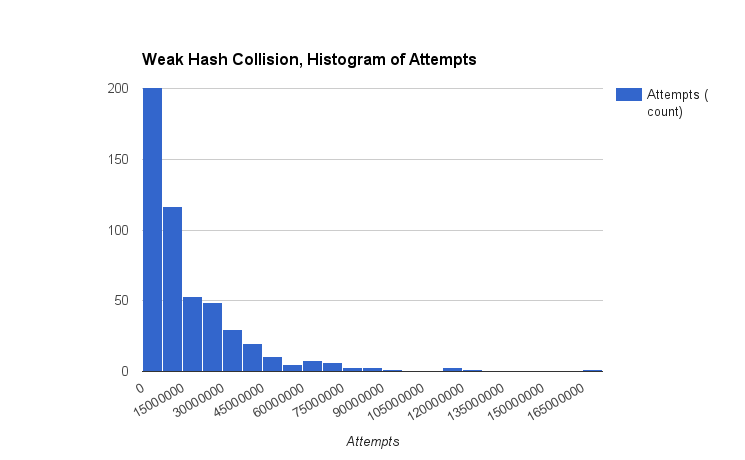
\includegraphics[scale=.5]{weak.png}

\subsection*{2}
Strong Hash Collision:\\
\noindent 500 Trials\\ Average Attempts: 5,370.812\\ Median Attempts: 4,911.5\\

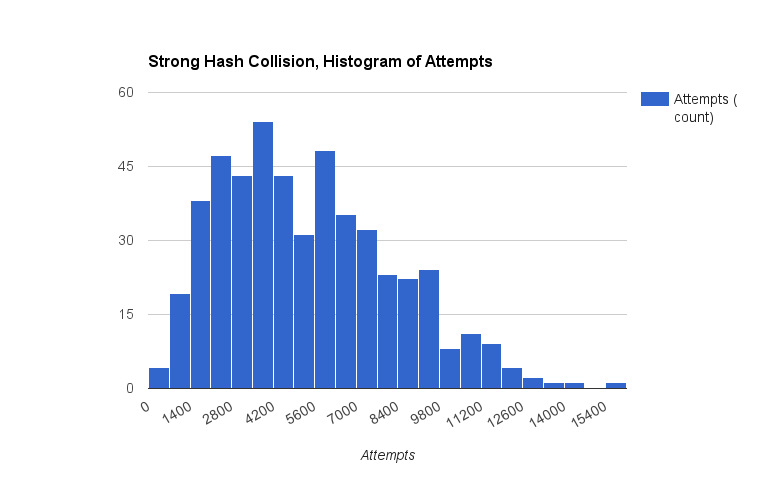
\includegraphics[scale=.5]{strong.png}

\subsection*{3}
Trial description: Each trial used a randomized string (strong) or a randomized
start hash (weak). \\

\noindent Overall, strong hash collision was much easier to break. Weak
hash collision on a three byte has took several million trials on average,
while a 3 byte hash took only about five thousand on average using strong hash
collision.\\

\noindent Mathematical description\\
\noindent Weak collision:\\
\noindent The probability of guessing a certain hash out of a 24 bit hash is the very
simple:\\

$Prob = 1/(2^{24}) = 1/16777216 = 5.9604 * 10^{-8}$\\\\

\noindent Strong collision:\\
\noindent For this equation, I'm plugging in the average number of attempts for n to give
a reasonable estimate of the probability:\\

$P(5370) = 1 - ((2^{24})!/((2^{24})^(5370)*(2^{24}-5370)!))$\\\\
$=.5765$\\

\noindent An incredibly large guessing chance for such a small number of attempts. 


\section*{Part 4}
From the CBC mode encryption, it's just noise. But from ECB, I can clearly see the outline
of Tux. While the colors are different, they are consistently different, allowing me
to make out the original picture with some alterations.\\ 


\includegraphics[scale=.1]{Tux.png}
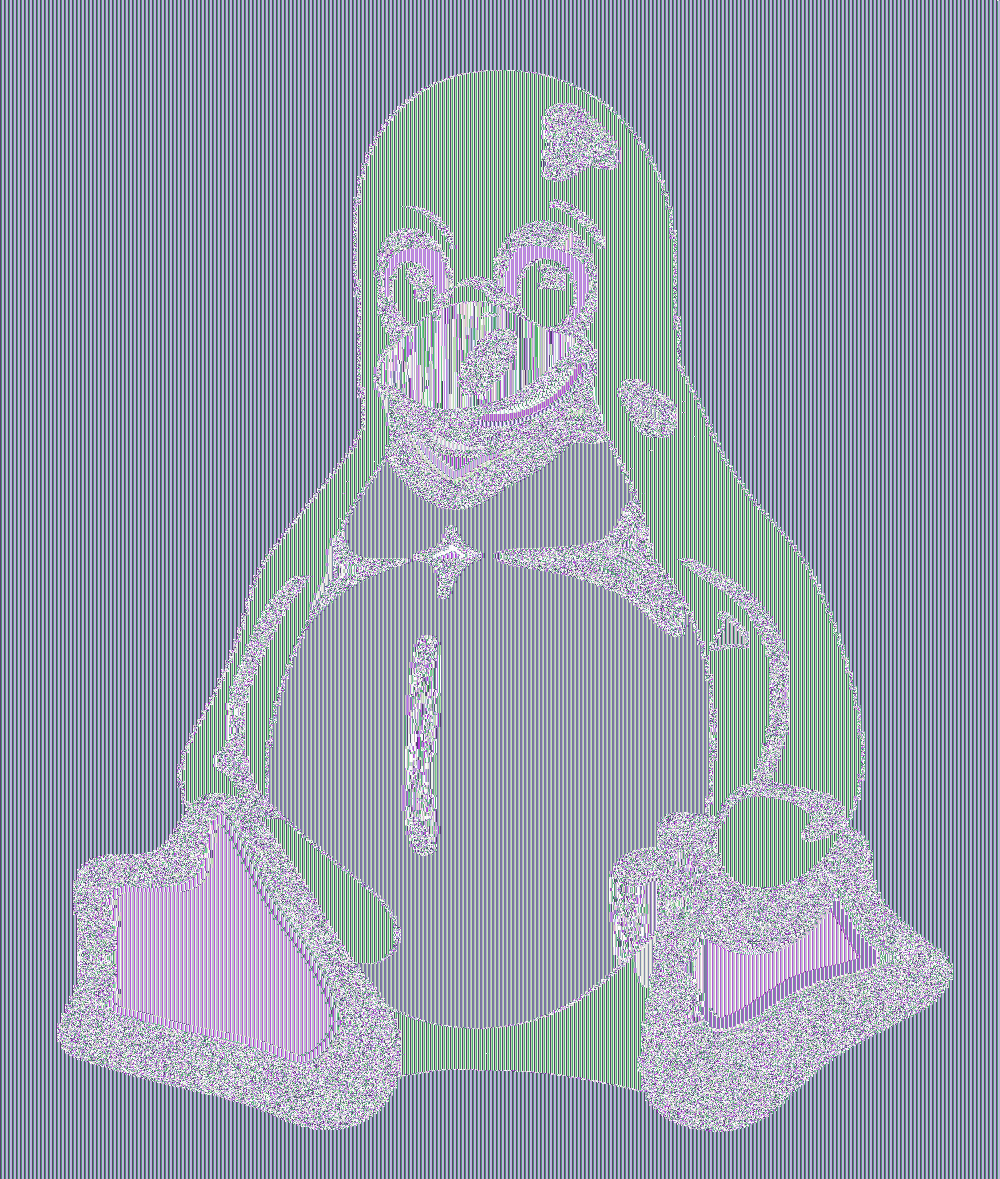
\includegraphics[scale=.1]{ecbtux.png}

\includegraphics[scale=.1]{cbctux.png}

\section*{Part 5}
My answer for the correct key is the word 'median'. I had some trouble on this part of the assignment.
Specifically, the hexadecimal conversion back and forth between strings. The other issue
I ran into was
my encryption function would only output the first half of the ciphertext correctly. I
piped the output of my program into a file, and grepped for the key we were provided.

\end{document}



